%% LyX 2.2.0alpha2 created this file.  For more info, see http://www.lyx.org/.
%% Do not edit unless you really know what you are doing.
\documentclass[english]{article}
\usepackage[T1]{fontenc}
\usepackage[latin9]{luainputenc}
\usepackage{geometry}
\geometry{verbose,tmargin=3cm,bmargin=3cm,lmargin=3cm,rmargin=3cm}
\usepackage{babel}
\usepackage{graphicx}
\usepackage{esint}
\usepackage[unicode=true]
 {hyperref}

\makeatletter

%%%%%%%%%%%%%%%%%%%%%%%%%%%%%% LyX specific LaTeX commands.
%% Because html converters don't know tabularnewline
\providecommand{\tabularnewline}{\\}

%%%%%%%%%%%%%%%%%%%%%%%%%%%%%% User specified LaTeX commands.
\usepackage{fancyheadings}
\pagestyle{fancy}
\lhead{Kellen Betts}
\chead{timeSeriesClassificationLDA}
\rhead{160731}

\makeatother

\begin{document}

\title{Classification of Time Series Data (e.g. Music)}

\author{Kellen Betts}

\date{Updated July 31, 2016}
\maketitle
\begin{abstract}
In this project an algorithm is developed to classify music genre
and bands based on their time-frequency signatures. An assortment
of music from my iTunes collection is used to build training sets
for band classification of bands from (1) different genres and (2)
the same genre, and (3) classification of different genres with assorted
bands. The computational methods used include time-frequency analysis
with the G�bor transform, singular value decomposition (SVD) to identify
dominant modes in the time-frequency data, and linear discriminant
analysis (LDA) to provide the classification metric. The results show
that this algorithm is most effective with band classification from
different genres with over an 80\% accuracy rate. Classification of
different genres and bands within a single genre show less promising
results with less than 70\% accuracy rates. The number of time-frequency
signatures (identified as modes from the SVD) necessary for optimal
classification is extensively explored with approximately ten modes
proving most effective.
\end{abstract}

\section{Introduction}

The objective in this project is to develop an algorithm that can
distinguish between music bands and genres. The basic components include
time-frequency analysis using the G�bor transform, singular value
decomposition (SVD) to identify dominant modes in the time-frequency
data, and linear discriminant analysis (LDA) to provide a classification
metric. An assortment of data from my iTunes collection is used to
build training sets and test the efficacy of the algorithm. The test
conditions used for this analysis were:
\begin{enumerate}
\item \textbf{Test 1} (Band Classification I): Three different bands from
\emph{different} genres. The bands used are Bob Marley (reggae), The
Offspring (modern or alternative rock), and Alireza Eftekhari (perhaps
best classified as ``international'').
\item \textbf{Test 2 }(Band Classification II): Three different bands from
the \emph{same} genre making separation much more difficult. The genre
used is modern or alternative rock and the bands used are Phish, Coldplay,
and Dave Matthews Band.
\item \textbf{Test 3} (Genre Classification): An assortment of bands from
three different genres are used to classify tracks by genre. The genres
used are classical, techno or electronica, and modern or alternative
rock with various bands 
\end{enumerate}

\section{Theoretical Background}

\subsection{Time-Frequency Analysis (G�bor)}

The basis used for time-frequency analysis in this project is the
G�bor transform. This technique is a windowed Fourier transform where
time and frequency components are identified. For a given function
$f(x)$ the Fourier transform and its inverse are defined,
\begin{equation}
F\left(k\right)=\frac{1}{\sqrt{2\pi}}\intop_{-\infty}^{\infty}e^{-ikx}f\left(x\right)dx
\end{equation}
\begin{equation}
f(x)=\frac{1}{\sqrt{2\pi}}\intop_{-\infty}^{\infty}e^{ikx}F(k)dk
\end{equation}
where $k$ corresponds to the wave-numbers in the trigonometric identity.
With the Fourier transform, the spectral content can be effectively
isolated from a signal but all temporal information is lost because
the signal is integrated over the domain $x\,\epsilon\,\left[-\infty,\infty\right]$
. The G�bor transform extends this technique by defining a time window
$g\left(\tau-t\right)$ that allows the transform to localize both
time and frequency content. For a given function $f\left(t\right)$
the G�bor transform is defined (Kutz 12.4.1),
\[
G\left[f\right]\left(t,\omega\right)=\intop_{-\infty}^{\infty}f\left(\tau\right)\bar{g}\left(\tau-t\right)e^{-i\omega\tau}d\tau\,.
\]
Computationally the G�bor transform is implemented over the finite
domains (Kutz 12.4.9a-b) 
\begin{equation}
\tau=b\,t_{0}
\end{equation}
\begin{equation}
v=a\,\omega_{0}
\end{equation}
 and so the discrete kernel for the transform becomes (Kutz 12.4.10),
\[
g_{m,n}\left(t\right)=e^{i2\pi a\omega_{0}t}g\left(t-b\,t_{0}\right)\,.
\]
Frequency content is isolated using the Fast Fourier Transform (FFT)
algorithm which can achieve a low operation count of $O\left(N\,\log N\right)$
assuming a $2^{n}$ discritization. Additionally, given its trigonometric
construction, the Fourier transform assumes a $2\pi$-periodic domain.

To filter the audio tracks, the first G�bor function used is a Gaussian
(Kutz 12.7.54),
\begin{equation}
g\left(t\right)=e^{-a\left(t-b\right)^{2}}
\end{equation}
where $a$ is the window width and $b$ is the length of the temporal
shift. The Gaussian is then compared to the Mexican Hat function defined
by (Kutz 12.5.24a),
\[
\psi\left(t\right)=\left(1-t^{2}\right)\exp\left(-\frac{t^{2}}{2}\right)
\]
which is implemented using the mother wavelet (Kutz 12.5.14),
\begin{equation}
\psi_{a,b}\left(t\right)=\frac{1}{\sqrt{a}}\,\psi\left(\frac{t-b}{a}\right)
\end{equation}
and so the function for the Mexican Hat Wavlet is given by,
\begin{equation}
\psi_{a,b}\left(t\right)=\frac{1}{\sqrt{a}}\,\left(1-\left(\frac{t-b}{a}\right)^{2}\right)\exp\left(-\frac{\left(\frac{t-b}{a}\right)^{2}}{2}\right).
\end{equation}


\subsection{Singular Value Decomposition}

The singular value decomposition (SVD) is defined,
\begin{equation}
X=U\Sigma V^{*}
\end{equation}
where $\Sigma$ is a diagonal matrix of singular values $\sigma$
that correspond to the square root of the eigenvalues $\left(\sigma_{i}=\sqrt{\lambda_{i}}\right)$
and are ordered based on size. $U$ and $V^{*}$ are orthonormal unitary
transformations corresponding to the orientation of the incoming data.
Using the proper orthogonal modes from the SVD, a low rank approximation
can be calculated by the sum,
\begin{equation}
X_{N}\approx\sum_{j=1}^{N}\sigma_{j}\vec{u}_{j}\vec{v^{*}}_{j}
\end{equation}
where $N$ is a given rank. The 2-norm error for the approximation
is given by,
\begin{equation}
\left\Vert X-X_{N}\right\Vert _{2}=\sigma_{n+1}\,.
\end{equation}
One way to think about SVD is as a least squares fit in higher dimensional
space where the elements of $\Sigma$ are ordered by their $L^{2}$
energy. The energy for a given mode can be calculated,
\begin{equation}
\mathrm{energy}_{i}=\frac{\sum_{i=1}^{N}\sigma_{i}}{\sum_{i=1}^{n}\sigma_{i}}\,.
\end{equation}
Therefore, diagonalization with SVD is a transformation to a new orthonormal
basis and provides low rank approximations for a given dataset.

\subsection{Linear Discriminate Analysis}

The central idea behind LDA is to ``find a suitable projection that
minimizes the distance between the inter-class data while minimizing
the intra-class data'' (Kutz p.378). This is achieved by the LDA
projector $\left(w\right)$,
\begin{equation}
w=\arg\max_{w}\frac{w^{T}S_{B}w}{w^{T}S_{W}w}
\end{equation}
The sample covariance of the class means is given by the inter-class
scatter matrix $\left(S_{B}\right)$ defined by (Wikipedia, \href{http://en.wikipedia.org/wiki/Linear_discriminant_analysis}{http://en.wikipedia.org/wiki/Linear\_{}discriminant\_{}analysis}),
\begin{equation}
S_{B}=\sum_{i=1}^{C}\left(\mu_{i}-\mu\right)\left(\mu_{i}-\mu\right)^{T}
\end{equation}
where $C$ is the number of classes (in this case 3), $\mu_{i}$ is
the mean for a given classes, and $\mu$ is the mean of the entire
dataset. The intra-class scatter matrix $\left(S_{W}\right)$ is defined
by,
\begin{equation}
S_{W}=\sum_{j=1}^{C}\sum_{x}\left(x-\mu_{j}\right)\left(x-\mu_{j}\right)^{T}
\end{equation}
For this analysis, the classes are the three bands or genres being
classified. The LDA projection vector is found by obtaining the eigenvector
of the maximum eigenvalue in the eigenvalue problem,
\begin{equation}
S_{B}w=\lambda S_{W}w\,.
\end{equation}


\section{Algorithm Implementation and Development}

The key steps in the algorithm are:
\begin{enumerate}
\item Build training data set:

\begin{enumerate}
\item Import music tracks
\item Gabor transform
\item SVD and LDA to provide test metric
\end{enumerate}
\item Test new tracks:

\begin{enumerate}
\item Import
\item Gabor transform
\item SVD and LDA projection
\item Classify results
\end{enumerate}
\end{enumerate}
The music used for this project was extracted from my iTunes music
collection. All of the tracks were preprocessed in an audio editing
application (\emph{Audacity}, \href{http://audacity.sourceforge.net/}{http://audacity.sourceforge.net/}).
Approximately 50 minutes of music for a given group (say Dave Matthews
Band or a mix of ``Classical'') were imported into a single file,
converted to a mono track (single channel), resampled at 8000 Hz,
and exported as a .wav file. In MATLAB loading and resampling of the
data is done in a subroutine ($\mathtt{loadTrack}$) where the full
.wav file is read in and 5 second samples are extracted randomly to
prevent bias in sampling. Random selection is implemented by using
a pseudo-random integer as the start point for extracting a 5 second
sample. Once imported, the sampling frequency for each track is reduced
to 2000 Hz (factor of 4) to reduce the size of the data and allow
more samples. Ideally, a large number of samples in each group would
be used for the training set. After exploring the parameters for this
algorithm, the optimal balance between reducing the sampling frequency,
increasing the number of samples, and preventing memory overload with
the SVD operation is 20 samples for each group meaning the full training
set has 60 tracks.

Once the tracks for the training set are imported, time-frequency
analysis is done using the G�bor transform algorithm developed for
Homework \#2. The algorithm is run in a subroutine ($\mathtt{gabor.m}$)
that processes a single track input, so a loop is run over the full
training set. The temporal domain is discritized with $n+1$ points
then trimmed to $n$ points since the FFT assumes periodic boundaries.
The frequency domain is discritized using, 
\begin{equation}
\mathtt{k=\frac{2\pi}{L}\left[0:(\frac{n}{2}-1)-\frac{n}{2}:-1\right]}
\end{equation}
which aligns with the shifted and $2\pi$-scaled domain of the FFT
algorithm. The Gaussian and Mexican Hat filter windows are implemented
as autonomous functions,
\begin{equation}
\mathtt{gaussian=@(a,b)exp(-a*(t-b).^{2})}
\end{equation}
\begin{equation}
\mathtt{mexHat=@(a,b)(1/sqrt(a))*(1-((t-b)/a).^{2}).*exp(-(((t-b)/a).^{2})/2)}
\end{equation}
Testing was done with the two filters and better results were obtained
with the Gaussian so it was selected for the analysis. Temporal sampling
is implemented using a linear vector that spans the length of the
temporal domain and is discritized to the sampling parameter $\left(b\right)$,
\begin{equation}
\mathtt{slide=linspace(t(1),t(end),b)}\,.
\end{equation}
The algorithm uses a loop for the temporal sampling in which the filter
function is applied to the track vector then transformed using the
FFT. Experimentation with the filter width $\left(a\right)$ and temporal
sampling $\left(b\right)$ was done to determine optimal values, and
$a=500$, $b=100$ were selected for the analysis. The data returned
by the $\mathtt{gabor.m}$ subroutine is shift from the FFT domain
and return in as a row vector.

After the full training set is processed using the G�bor transform,
the data is then sent to a subroutine ($\mathtt{trainer.m}$) that
implements the SVD and linear discriminant analysis. A reduced SVD
is computed using the built-in MATLAB function which returns the $U$,
$S$, and $V$ matrices. The principal components are calculated for
a given number of ``features'' or modes. (The orientation of the
training data that was more efficient for the SVD function meant the
principal components were calculated $SU^{T}$.) From the principal
components, means are calculated for each group and the scatter matrices
$S_{b}$ and $S_{w}$ are built. Next the eigenvalue problem (equation
15) is solved using the built-in MATLAB function $\mathtt{eig}$ and
the maximum eigenvalue and corresponding eignevector (LDA projector
$w$) are found. Finally, the principal components for each group
in the training set are projected on the LDA projector $\left(w\right)$
and means for each group are calculated. The $\mathtt{trainer.m}$
subroutine then returns the results from both the SVD and LDA for
further analysis.

The tracks that are used to test the LDA training set are imported
and processed by the G�bor transform in the same manner as the training
data. This analysis used 10 tracks from each group (30 tracks total)
for testing. The resulting time-frequency data is then projected onto
the SVD components using the $V^{T}$ obtained from the SVD and subsequent
LDA projector $\left(w\right)$ from the training set. Classification
of a selected track is then done by comparing the projection values
to the groups means from the train set with the closest value used.

Exploration of the ``features'' (modes from the SVD/LDA) is done
by running the with 1, 2, 4, 6, 8, 10, 20, 30, 40, 50, and 60 (full
rank) features. Accuracy rates are averaged over 9 trials for each
value of the parameter to get a better estimate of the performance
of the algorithm given the pseudo-random sampling procedure. The accuracy
rate is calculated as a percent correct where 100\% perfect performance.
Means and standard deviations are reported and discussed in Section
4 (Computational Results), and the full data set is available in Appendix
D.

\section{Computational Results}

\subsection{Test 1}

The objective of this test is to build a train set for three different
bands from three different genres of music. The test is to see if
the algorithm can classify new songs from the bands correctly. The
three bands used are Bob Marley (reggae), The Offspring (modern or
alternative rock), and Alireza Eftekhari (perhaps best classified
as ``international''). As seen in Figure 1, the original audio data
from these three groups have distinct audio signatures. SVD of the
time-frequency content shows (Figure 2) that the first mode is dominant
but there is a clear heavy-tail distribution of the singular values.
Spectrograms of the first four principal components (Figure 3) shows
distinct time-frequency signatures for each component. Projection
of the individual tracks onto the first three POD modes (Figure 4)
shows shows high intra-band variance and distinct signatures between
the groups\textbf{.} Figure 5 shows histograms of the projections
confirming the high intra-band variance and distinct signatures for
each band.

The results are summarized in Table 1. The averages (over 9 trials)
indicate that the algorithm is near 80\% accuracy for almost all modes.
Peak performance at over 80\% accuracy is seen with the 6, 8, and
10 rank projections. High deviations (particularly with higher rank
projections) confirming the variability within a given group as seen
in the projections (Figure 4). Since pseudo-random sampling is used
to extract the track data it is possible that some of the samples
may have contain little or no ``musical'' content (i.e. sampling
at the beginning or end of a song). Nonetheless, these results strongly
suggest that the algorithm was able to achieve over 80\% accuracy
for band classification with low rank approximations.

\pagebreak{}

\noindent \begin{center}
\begin{tabular}{|c|c|c|}
\hline 
\textbf{\# of Features} & \textbf{Accuracy (Mean)} & \textbf{Std. Dev.}\tabularnewline
\hline 
\hline 
1 & 77\% & 7.5\%\tabularnewline
\hline 
2 & 66\% & 11.8\%\tabularnewline
\hline 
4 & 79\% & 10.3\%\tabularnewline
\hline 
6 & 82\% & 9.9\%\tabularnewline
\hline 
8 & 81\% & 10.6\%\tabularnewline
\hline 
10 & 83\% & 7.2\%\tabularnewline
\hline 
20 & 76\% & 15.8\%\tabularnewline
\hline 
30 & 75\% & 11.9\%\tabularnewline
\hline 
40 & 74\% & 13.0\%\tabularnewline
\hline 
50 & 68\% & 16.2\%\tabularnewline
\hline 
60 & 58\% & 12.0\%\tabularnewline
\hline 
\end{tabular}
\par\end{center}

\noindent \begin{center}
\textbf{}%
\begin{minipage}[t]{0.75\columnwidth}%
\textbf{Table 1.} For Test 1, mean and standard deviation results
from 9 trials at the given values of the ``features'' parameter.''
The algorithm has an over 80\% accuracy rate for classification of
bands in different genres.%
\end{minipage}\vspace{0.1\paperheight}
\par\end{center}

\noindent \begin{center}
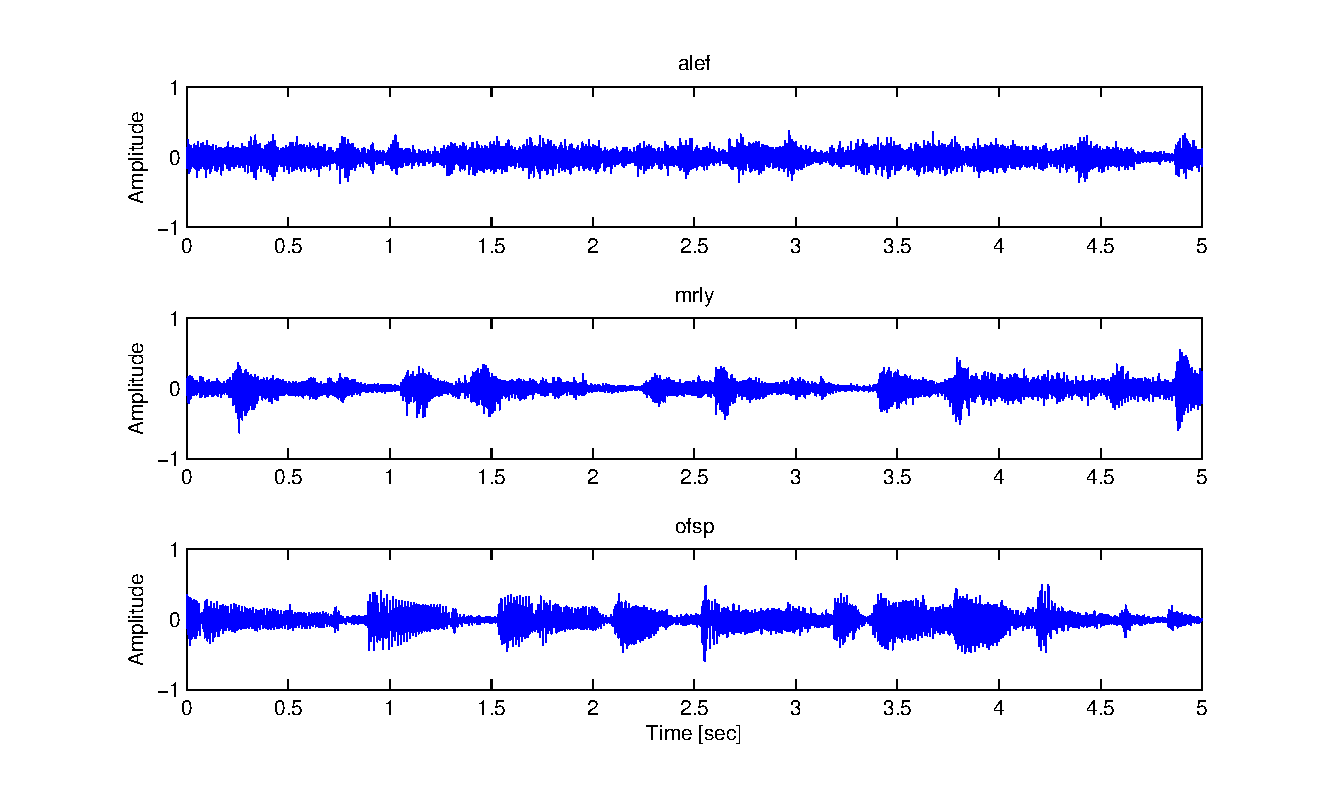
\includegraphics[width=0.95\columnwidth]{plot/test1/originals}\textbf{}\\
\textbf{}%
\begin{minipage}[t]{0.75\columnwidth}%
\textbf{Figure 1.} For Test 1, samples of the original audio show
that the three groups Alireza Eftekhari (top), Bob Marley (center),
and The Offspring (bottom) have distinct audio signatures.%
\end{minipage}
\par\end{center}

\noindent \begin{center}
\pagebreak{}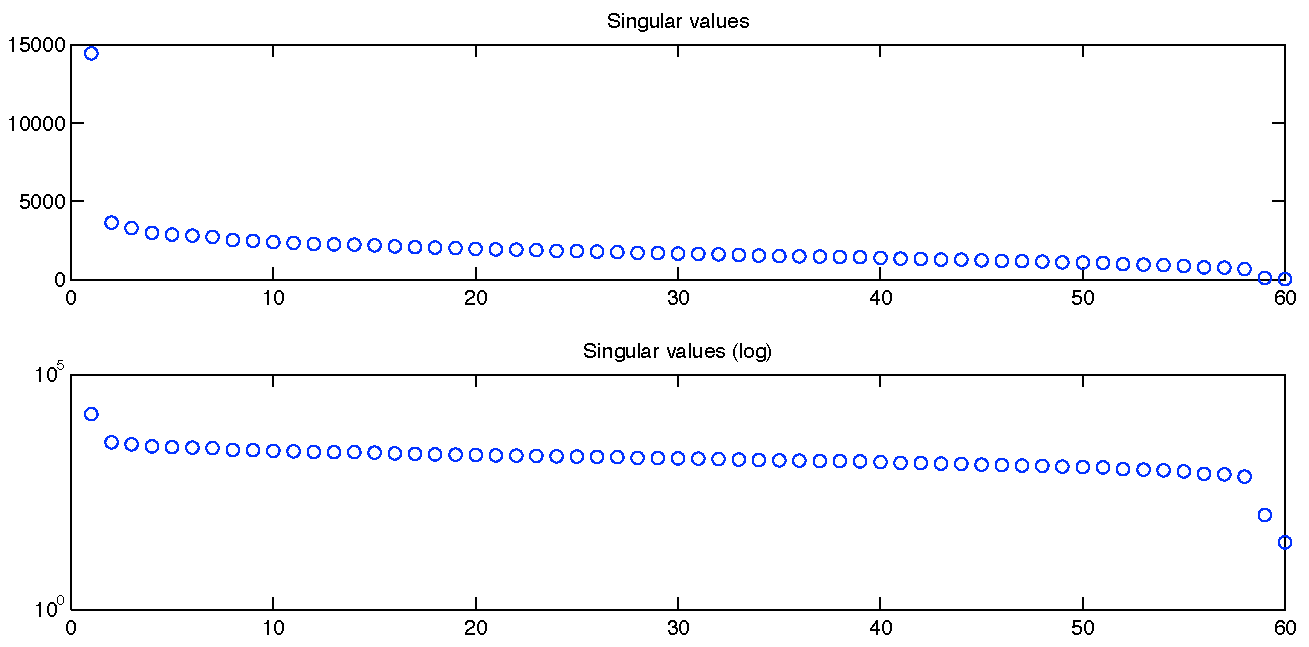
\includegraphics[width=0.85\columnwidth]{plot/test1/singVals}\textbf{}\\
\textbf{}%
\begin{minipage}[t]{0.75\columnwidth}%
\textbf{Figure 2.} For Test 1, the first singular value is dominant,
but there is a clear heavy-tail distribution.%
\end{minipage}\vspace{0.1\paperheight}
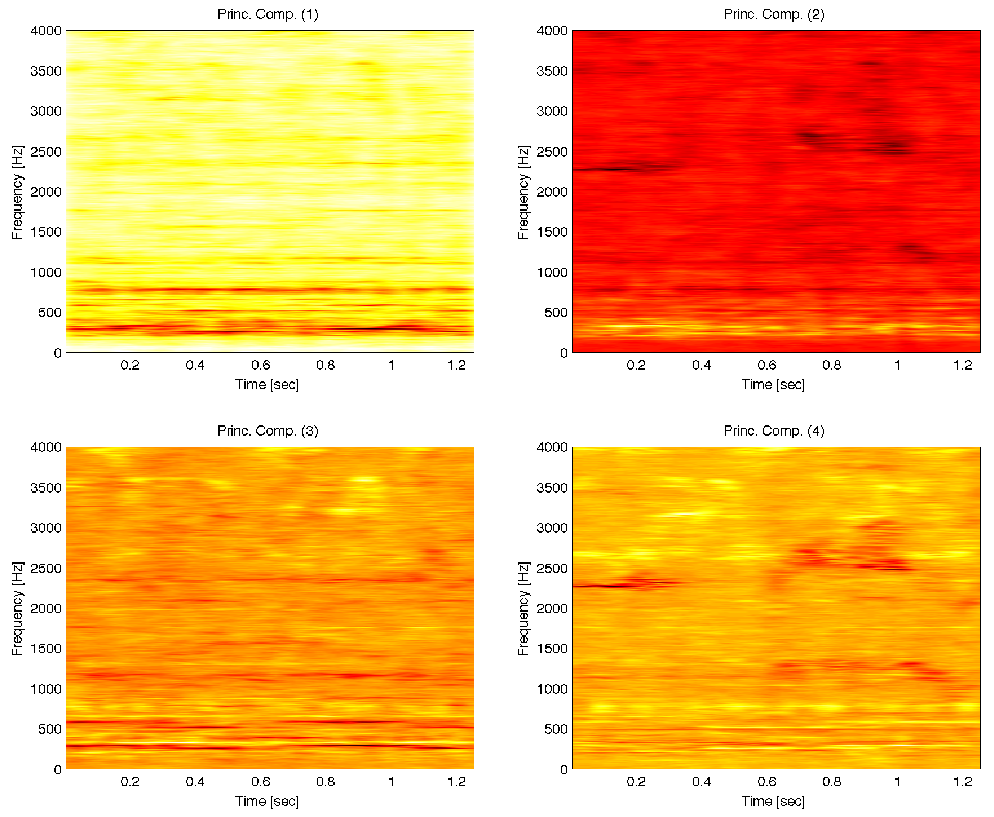
\includegraphics[width=0.75\columnwidth]{plot/test1/prinComp}\textbf{}\\
\textbf{}%
\begin{minipage}[t]{0.75\columnwidth}%
\textbf{Figure 3.} For Test 1, the first four principal components
show distinct time-frequency signatures.%
\end{minipage}
\par\end{center}

\noindent \begin{center}
\pagebreak{}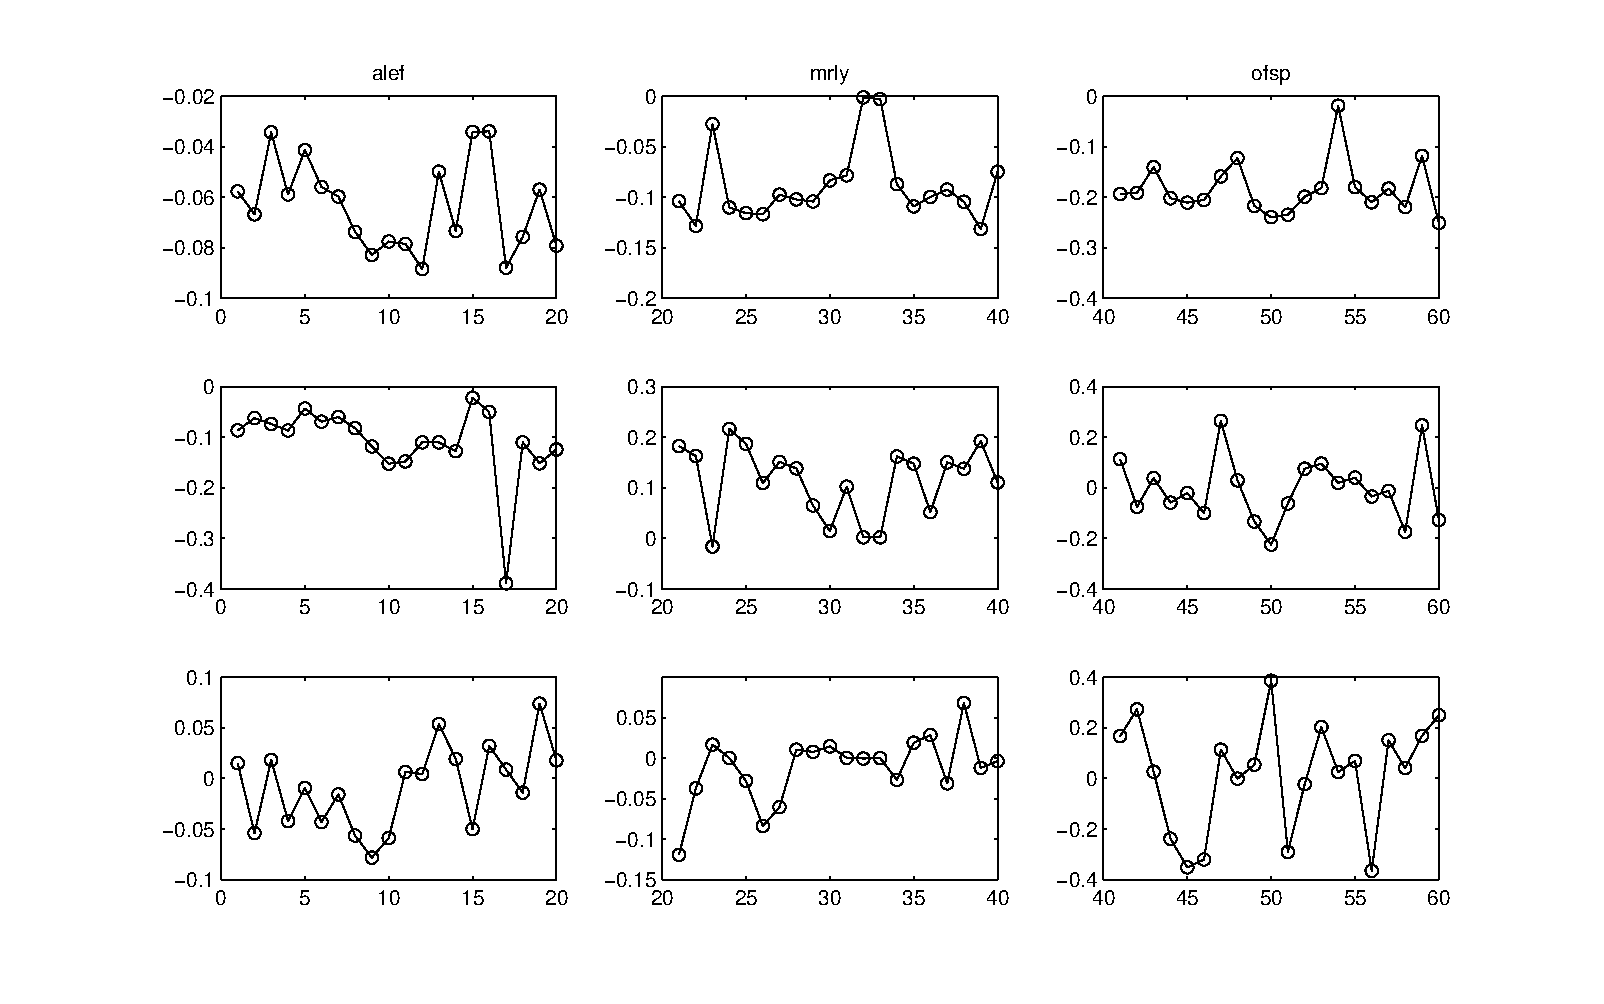
\includegraphics[width=0.95\columnwidth]{plot/test1/projections}\textbf{}\\
\textbf{}%
\begin{minipage}[t]{0.75\columnwidth}%
\textbf{Figure 4.} For Test 1, projection of the individual tracks
onto the first three POD modes shows high intra-band variance and
distinct signatures for each group: Alireza Eftekhari (left), Bob
Marley (center), and The Offspring (right).%
\end{minipage}\vspace{0.1\paperheight}
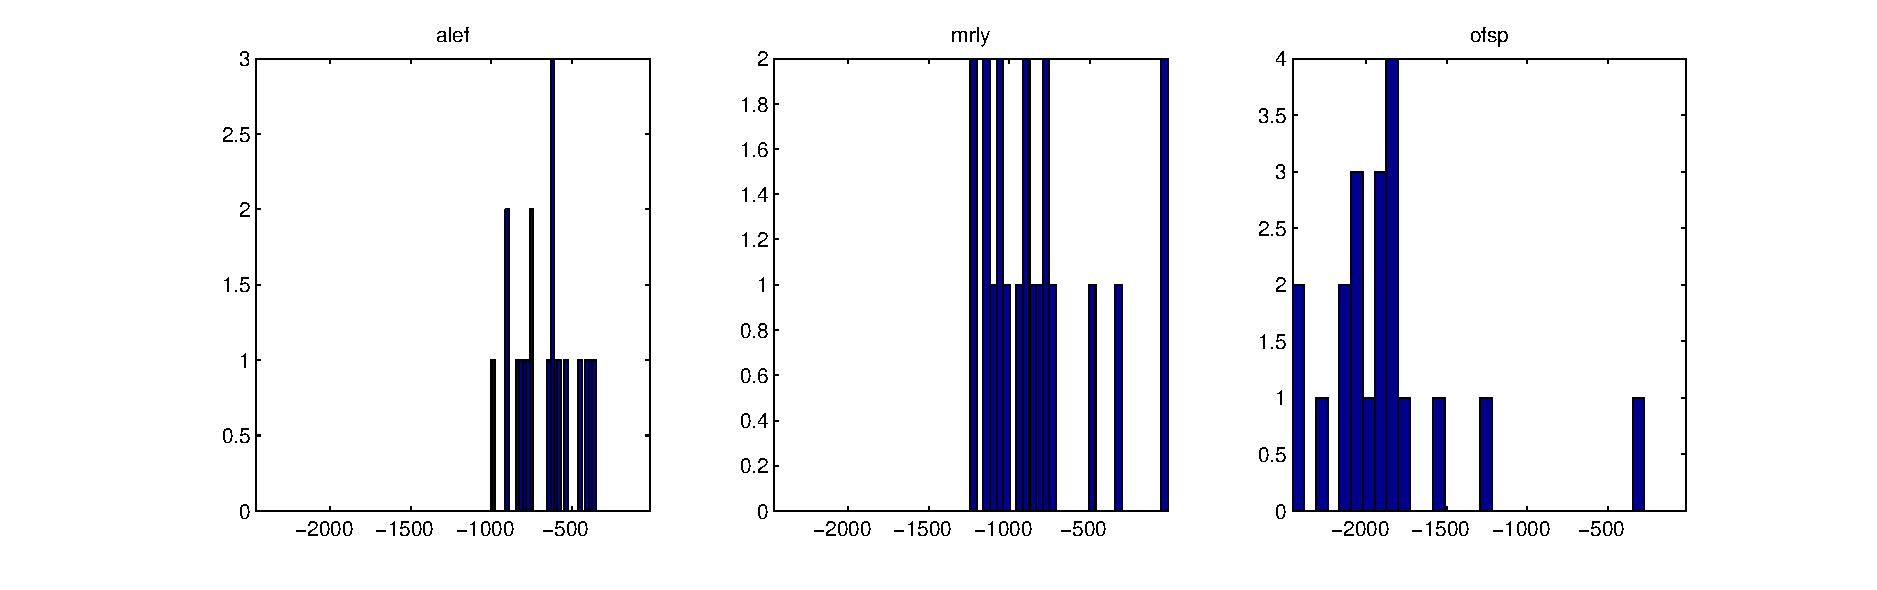
\includegraphics[width=0.95\columnwidth]{plot/test1/histogram}\textbf{}\\
\textbf{}%
\begin{minipage}[t]{0.75\columnwidth}%
\textbf{Figure 5.} For Test 1, histograms of the projections shows
high intra-band variance and distinct signatures for each band: Alireza
Eftekhari (left), Bob Marley (center), and The Offspring (right).%
\end{minipage}\pagebreak{}
\par\end{center}

\subsection{Test 2}

The objective of this test is to classify bands within a single genre
(modern or alternative rock). This is a much more difficult test condition
because within a genre there is much less variance between the bands
than the first test condition. The music tested is from Phish, Coldplay,
and Dave Mathews Band. As seen in Figure 6, the samples of the original
audio is very similar for both Phish and Dave Matthews, and the track
from Coldplay is the only one with notable visual difference. As with
the first test condition there is a clear heavy-tail distribution
of the singular values (Figure 7) but the first mode is still dominant.
Spectrograms of the first four principal components (Figure 8) show
distinct time-frequency signatures for each component. Projection
of the individual tracks onto the first three POD modes (Figure 9)
shows distinct signatures for each group and high intra-band variance.
The histograms in Figure 10 confirms the high intra-band variance,
and shows that Coldplay and Dave Matthews are similar and Phish is
notable different.

The results in Table 2 indicate the algorithm has approximately 60\%
accuracy, which is not that much better than random selection (50-50).
Peak performance at 66\% is seen with 8 features. As in the previous
test condition, the high deviations confirm the variability within
a given group. These results suggest the algorithm has the potential
to classify bands from the same genre, but is not achieving optimal
performance with the training set and parameters used in this analysis.\vspace{0.01\paperheight}

\noindent \begin{center}
\begin{tabular}{|c|c|c|}
\hline 
\textbf{\# of Features} & \textbf{Accuracy (Mean)} & \textbf{Std. Dev.}\tabularnewline
\hline 
\hline 
1 & 57\% & 7.0\%\tabularnewline
\hline 
2 & 60\% & 9.0\%\tabularnewline
\hline 
4 & 54\% & 15.1\%\tabularnewline
\hline 
6 & 63\% & 14.9\%\tabularnewline
\hline 
8 & 66\% & 11.6\%\tabularnewline
\hline 
10 & 63\% & 10.3\%\tabularnewline
\hline 
20 & 64\% & 10.1\%\tabularnewline
\hline 
30 & 61\% & 8.7\%\tabularnewline
\hline 
40 & 60\% & 5.9\%\tabularnewline
\hline 
50 & 61\% & 6.5\%\tabularnewline
\hline 
60 & 44\% & 13.1\%\tabularnewline
\hline 
\end{tabular}
\par\end{center}

\noindent \begin{center}
\textbf{}%
\begin{minipage}[t]{0.75\columnwidth}%
\textbf{Table 2.} For Test 2, mean and standard deviation results
from 9 trials at the given values of the ``features'' parameter.''
The algorithm has an over 63\% accuracy rate for classification of
bands in the same genre.%
\end{minipage}\pagebreak{}
\par\end{center}

\noindent \begin{center}
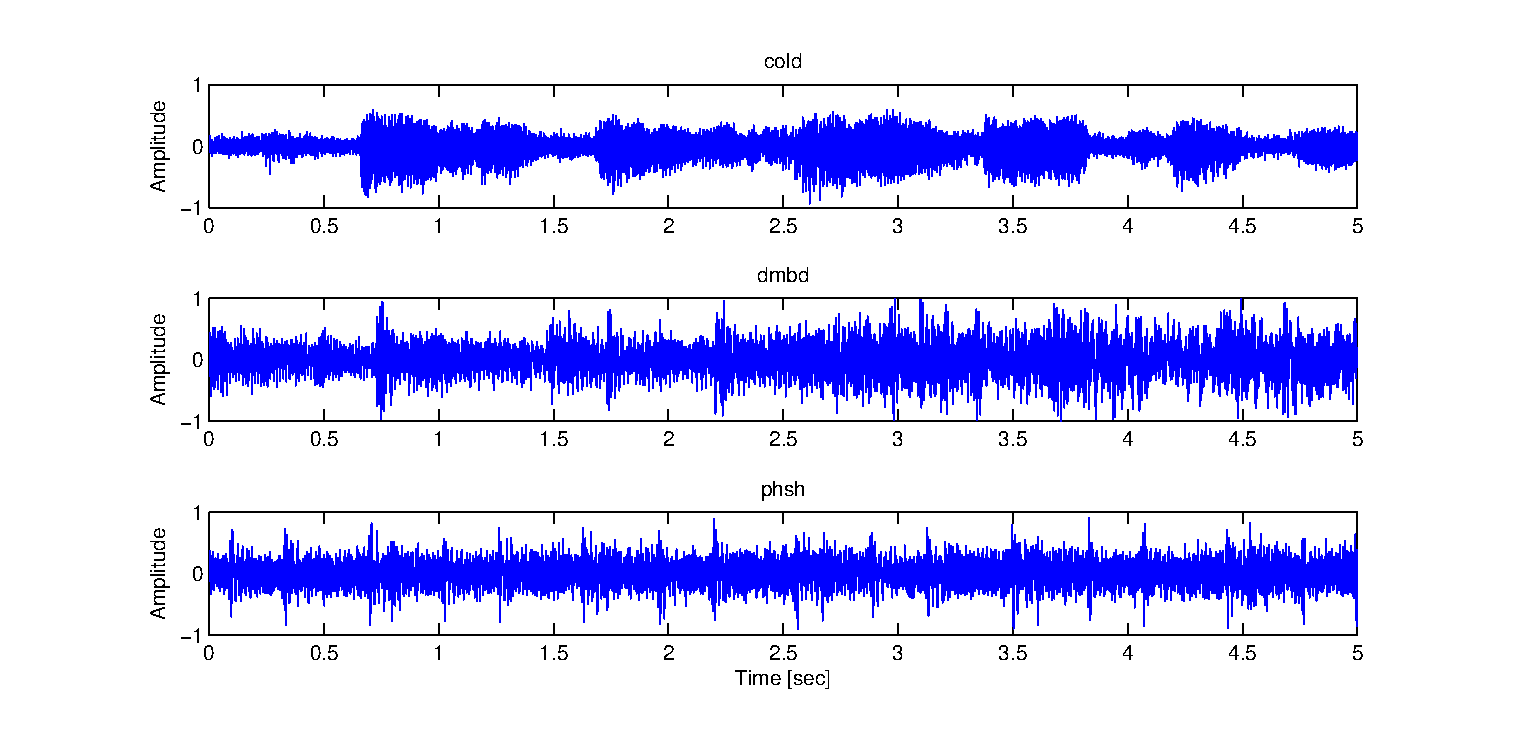
\includegraphics[width=0.95\columnwidth]{plot/test2/originals}\textbf{}\\
\textbf{}%
\begin{minipage}[t]{0.75\columnwidth}%
\textbf{Figure 6.} For Test 2, samples of the original audio show
that Phish (bottom) and Dave Matthews (center) are very similar, and
the track from Coldplay (top) is the only one with notable visual
difference%
\end{minipage}\vspace{0.07\paperheight}
\par\end{center}

\noindent \begin{center}
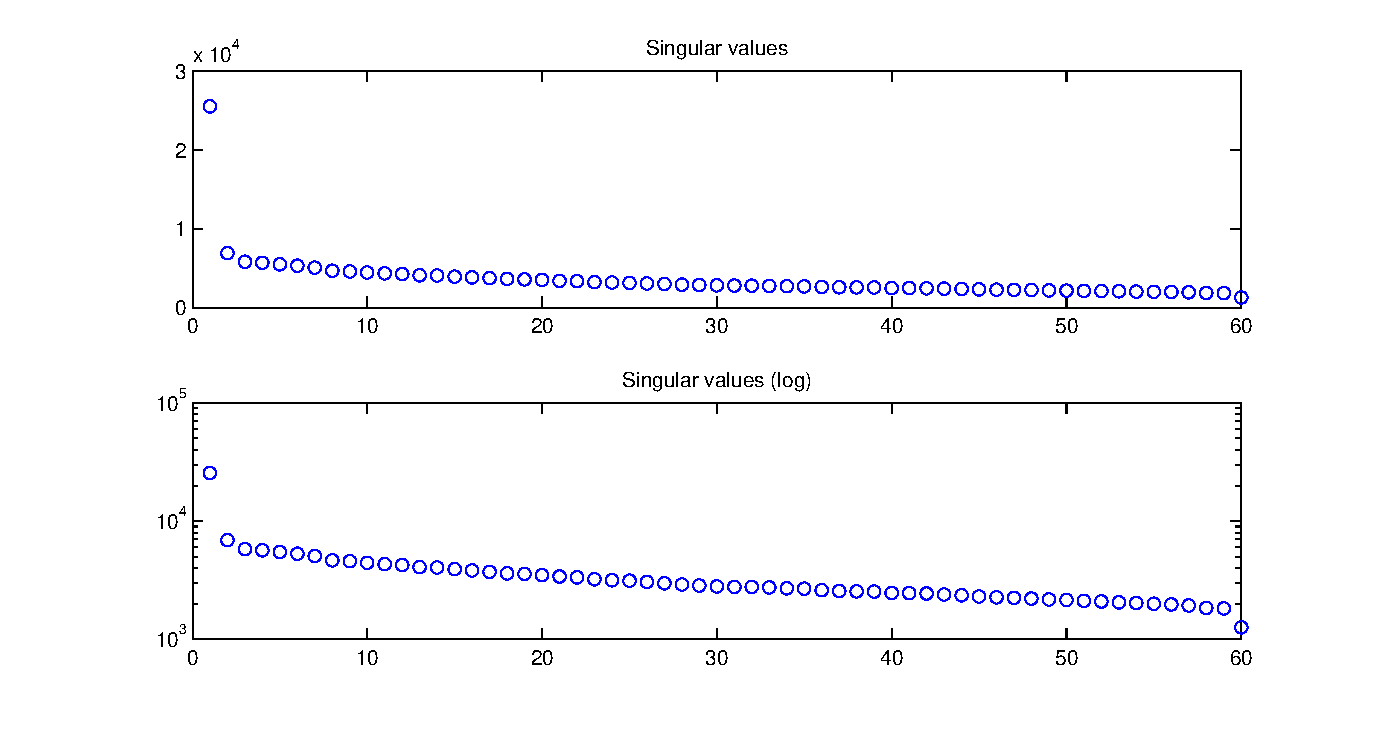
\includegraphics[width=0.85\columnwidth]{plot/test2/singVals}\textbf{}\\
\textbf{}%
\begin{minipage}[t]{0.75\columnwidth}%
\textbf{Figure 7.} For Test 2, the first singular value is dominant,
but there is a clear heavy-tail distribution.%
\end{minipage}
\par\end{center}

\noindent \begin{center}
\pagebreak{}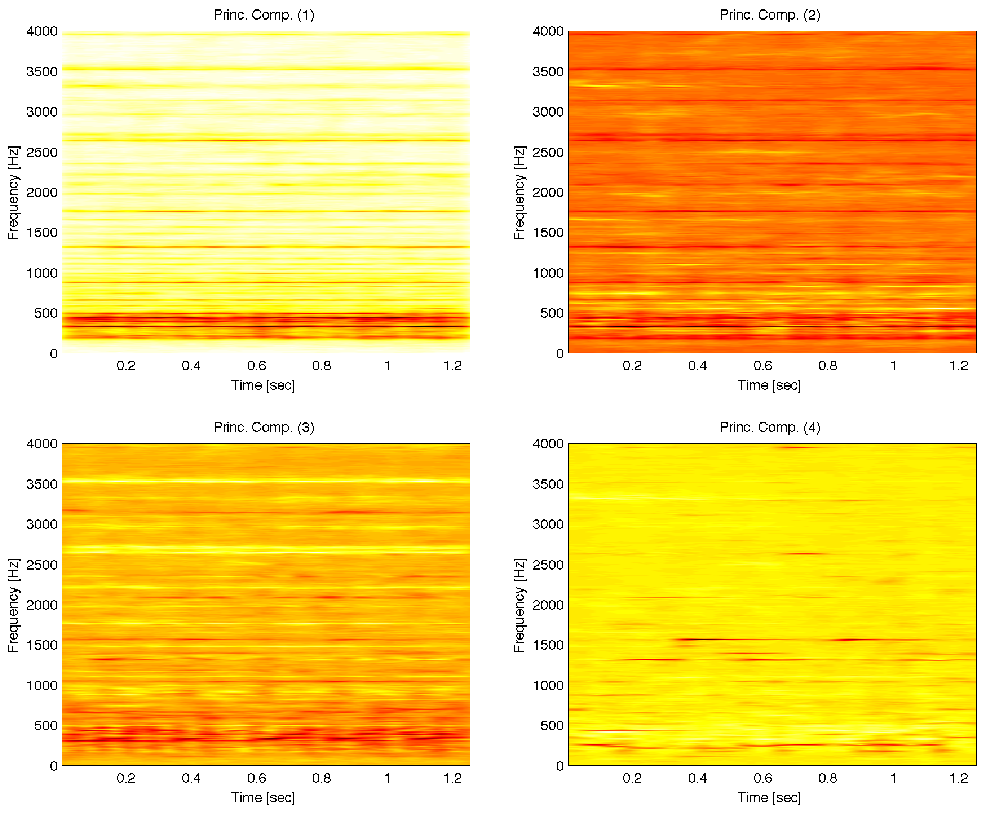
\includegraphics[width=0.75\columnwidth]{plot/test2/prinComp}\textbf{}\\
\textbf{}%
\begin{minipage}[t]{0.75\columnwidth}%
\textbf{Figure 8.} For Test 2, the first four principal components
show distinct time-frequency signatures.%
\end{minipage}\vspace{0.05\paperheight}
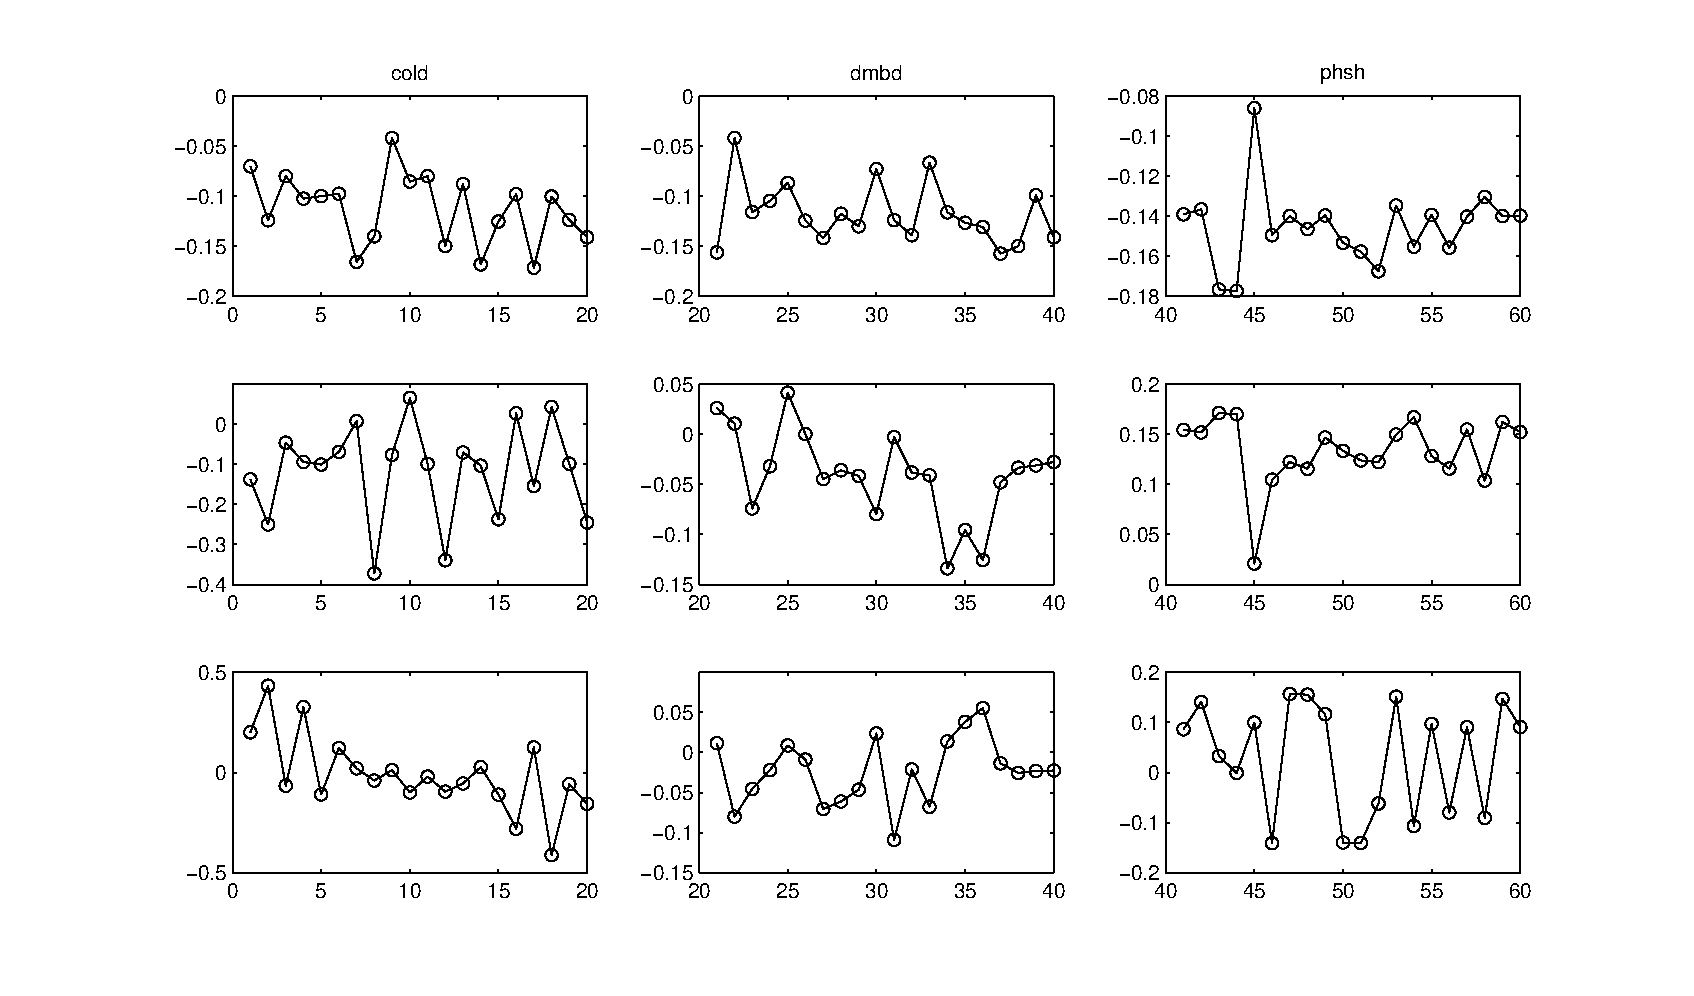
\includegraphics[width=0.85\columnwidth]{plot/test2/projections}\textbf{}\\
\textbf{}%
\begin{minipage}[t]{0.75\columnwidth}%
\textbf{Figure 9.} For Test 2, projection of the individual tracks
onto the first three POD modes shows high intra-band variance and
distinct signatures for each group: Coldplay (left), Dave Matthews
(center), and Phish (right).%
\end{minipage}
\par\end{center}

\noindent \begin{center}
\pagebreak{}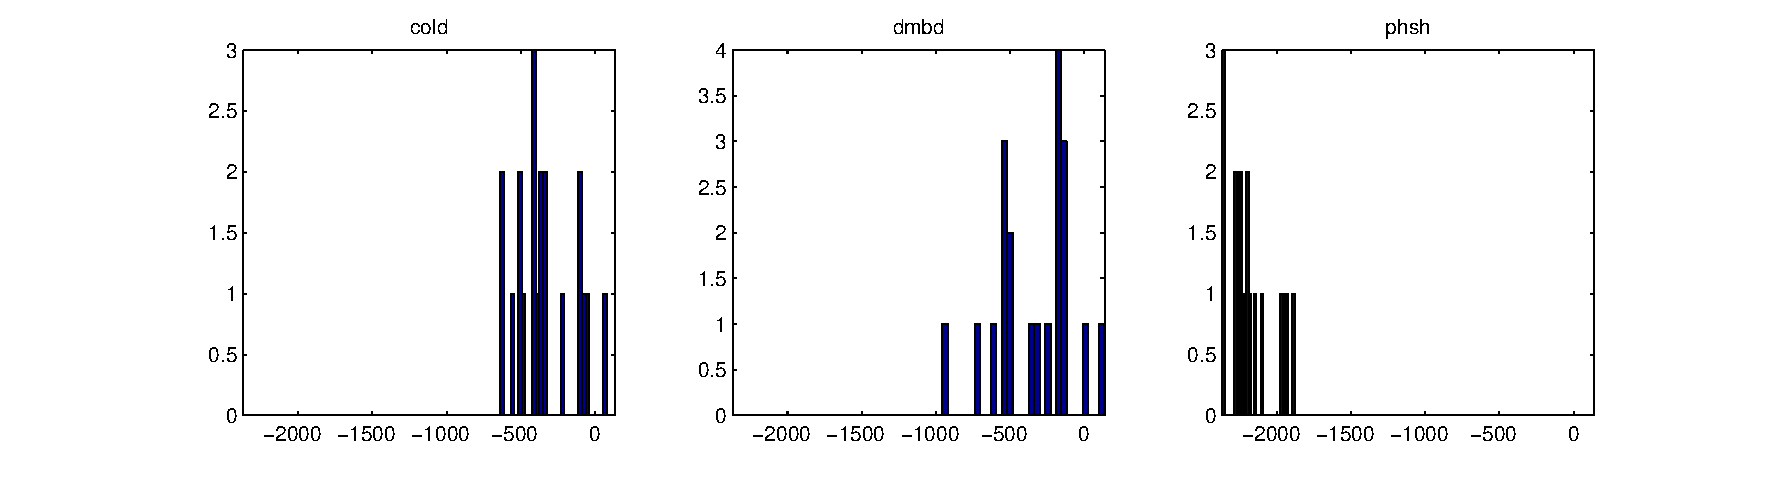
\includegraphics[width=0.95\columnwidth]{plot/test2/histogram}\textbf{}\\
\textbf{}%
\begin{minipage}[t]{0.75\columnwidth}%
\textbf{Figure 10.} For Test 2, histograms of the projections shows
high intra-band variance, that Coldplay (left) and Dave Matthews (center)
are similar and Phish (left) is notable different.%
\end{minipage}\vspace{0.02\paperheight}
\par\end{center}

\subsection{Test 3}

The objective of this test is to classify musical genres using a selection
of bands within each genre. The three genres that tested are classical
(Beethoven, Chopin, Rachmaninov, Mozart, and others), modern or alternative
rock (Phish, Coldplay, Dave Mathews Band, and others) and techno (Fat
Boy Slim, The Chemical Brothers, Moby, Yello, and others). As seen
in Figure 13, the samples of the original audio show the three genres
have the most distinct audio signatures in all the tests. As with
the previous tests, the first singular value is still dominant but
there is a clear heavy-tail distribution of the singular values (Figure
15). Spectrograms of the first four principal components (Figure 16)
show distinct time-frequency signatures for each component. Projection
of the individual tracks onto the first three POD modes (Figure 17)
show high intra-genre variance as seen in the previous tests and distinct
signatures for each genre. The histograms of the projections in Figure
18 confirms the high intra-genre variance, but also shows distinct
signatures for each genre.

The results in Table 3 indicate the algorithm has approximately 65\%
accuracy, similar to test 2. Peak performance at 68\% is seen with
10 features. As in the discussed previously, the deviations are high,
but in this test they are consistently lower than the previous test
conditions suggesting more accuracte results for this test. However,
similar to Test 2 these results indicate the algorithm has the potential
classify genres, but is not achieving optimal performance with the
training set and parameters used in this analysis. \vspace{0.01\paperheight}

\noindent \begin{center}
\begin{tabular}{|c|c|c|}
\hline 
\textbf{\# of Features} & \textbf{Accuracy (Mean)} & \textbf{Std. Dev.}\tabularnewline
\hline 
\hline 
1 & 64\% & 6.5\%\tabularnewline
\hline 
2 & 64\% & 7.2\%\tabularnewline
\hline 
4 & 64\% & 9.8\%\tabularnewline
\hline 
6 & 65\% & 9.1\%\tabularnewline
\hline 
8 & 67\% & 6.9\%\tabularnewline
\hline 
10 & 68\% & 7.1\%\tabularnewline
\hline 
20 & 67\% & 7.0\%\tabularnewline
\hline 
30 & 66\% & 8.3\%\tabularnewline
\hline 
40 & 67\% & 9.2\%\tabularnewline
\hline 
50 & 62\% & 9.2\%\tabularnewline
\hline 
60 & 54\% & 12.8\%\tabularnewline
\hline 
\end{tabular}
\par\end{center}

\noindent \begin{center}
\textbf{}%
\begin{minipage}[t]{0.75\columnwidth}%
\textbf{Table 3.} For Test 3, mean and standard deviation results
from 9 trials at the given values of the ``features'' parameter.''
The algorithm has an over 67\% accuracy rate for classification of
different genres.%
\end{minipage}\pagebreak{}
\par\end{center}

\noindent \begin{center}
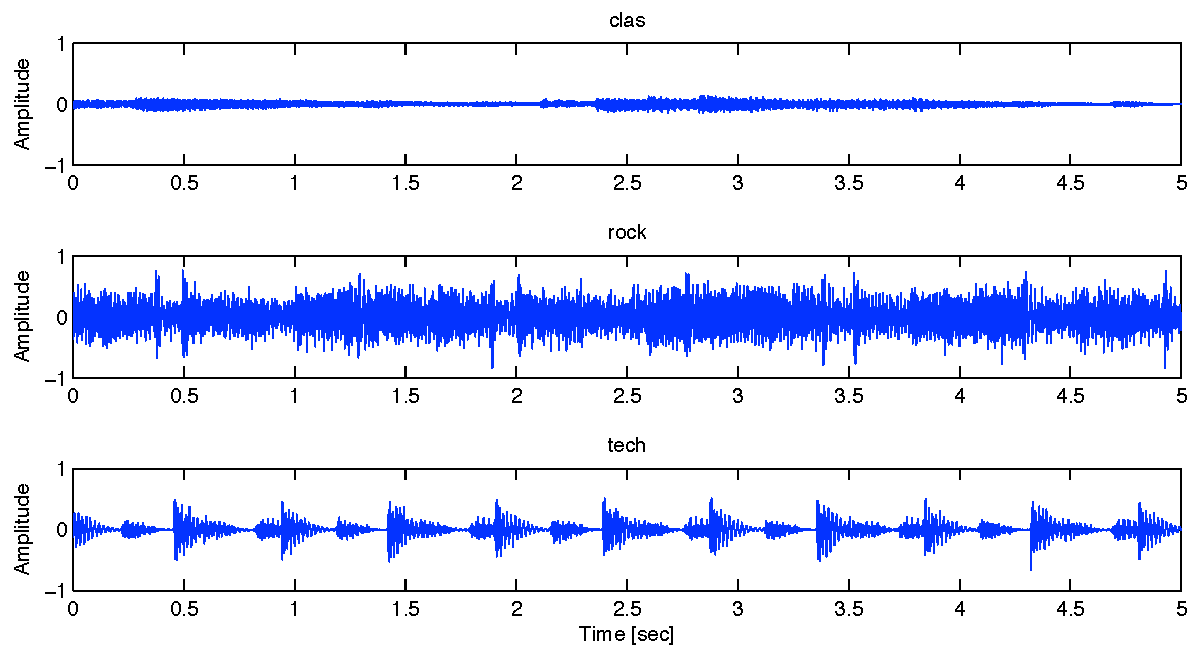
\includegraphics[width=0.95\columnwidth]{plot/test3/originals}\textbf{}\\
\textbf{}%
\begin{minipage}[t]{0.75\columnwidth}%
\textbf{Figure 11.} For Test 3, samples of the original audio show
that the three genres classical (top), modern rock (center), and techno
(bottom) have the most distinct audio signatures in all the tests.%
\end{minipage}\vspace{0.1\paperheight}
\par\end{center}

\noindent \begin{center}
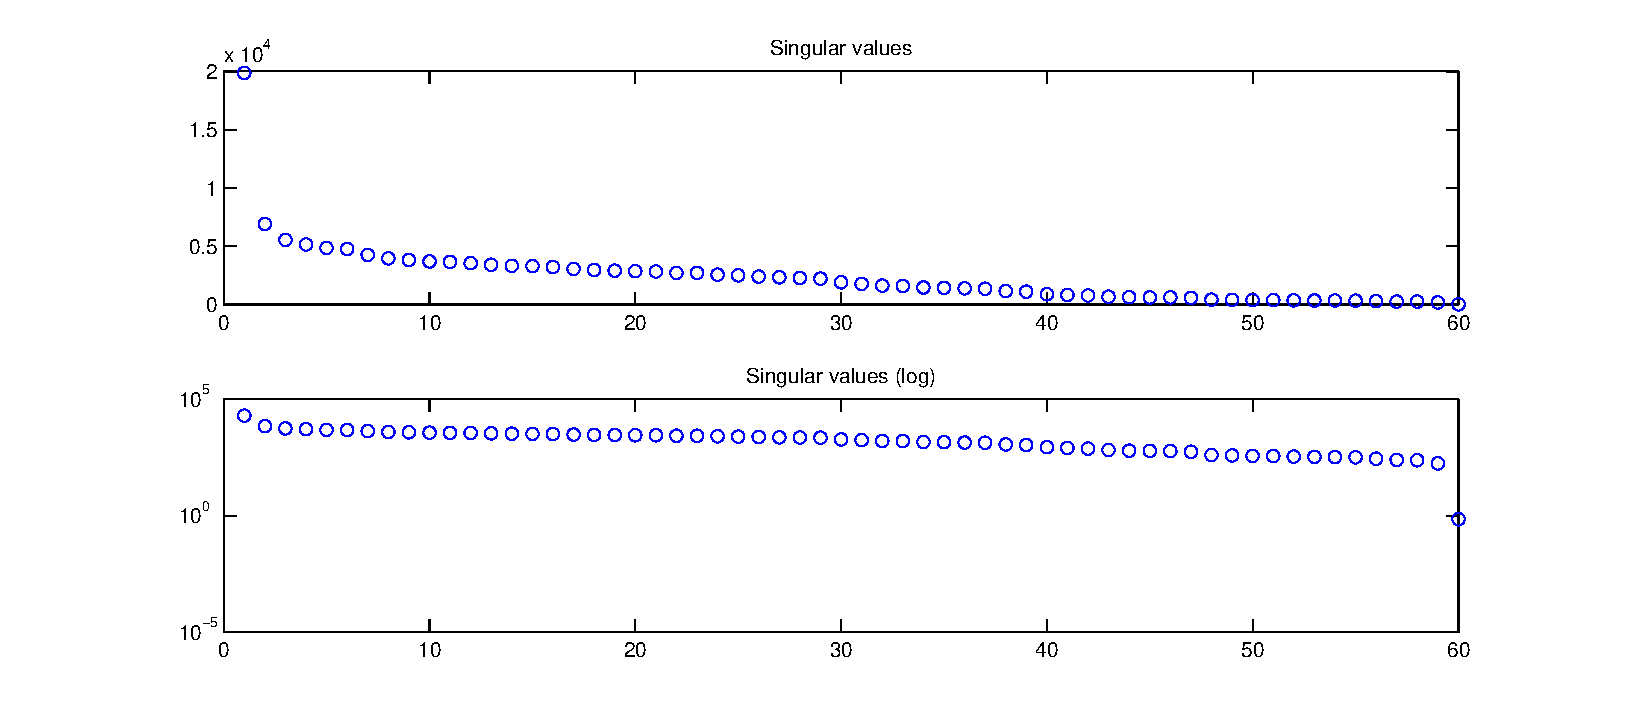
\includegraphics[width=0.85\columnwidth]{plot/test3/singVals}\textbf{}\\
\textbf{}%
\begin{minipage}[t]{0.75\columnwidth}%
\textbf{Figure 12.} For Test 3, the first singular value is still
dominant, and there is still a clear heavy-tail distribution.%
\end{minipage}
\par\end{center}

\noindent \begin{center}
\pagebreak{}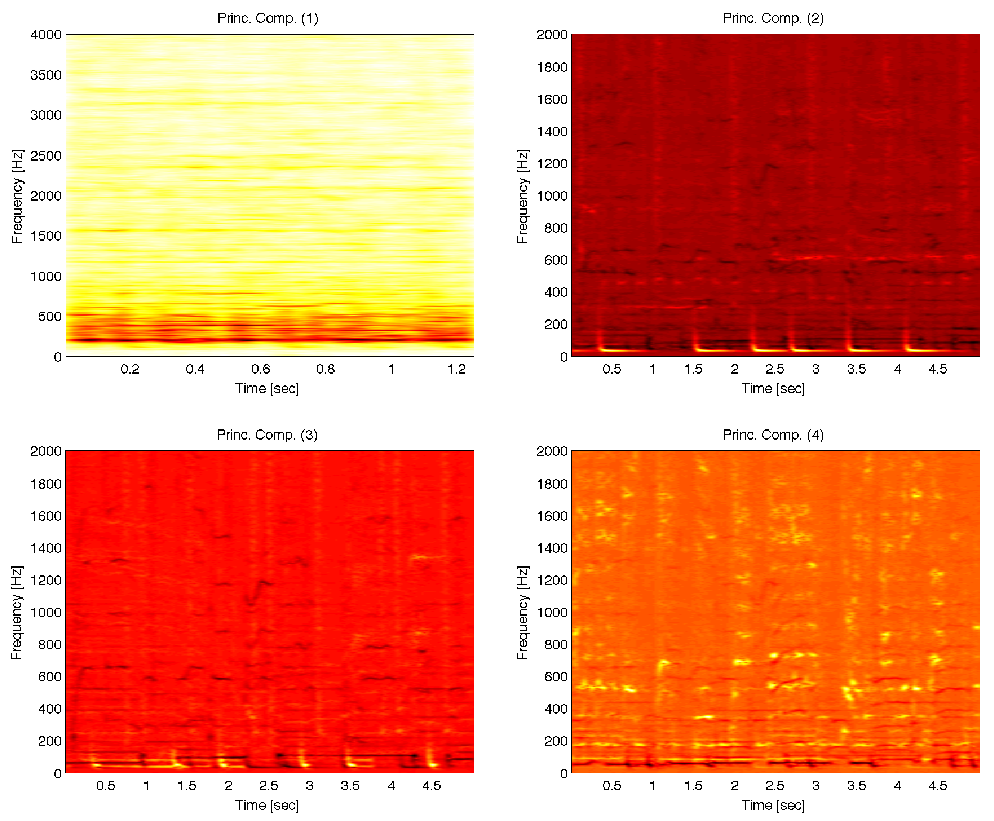
\includegraphics[width=0.75\columnwidth]{plot/test3/prinComp}\textbf{}\\
\textbf{}%
\begin{minipage}[t]{0.75\columnwidth}%
\textbf{Figure 13.} For Test 3, the first four principal components
show distinct time-frequency signatures.%
\end{minipage}\vspace{0.02\paperheight}
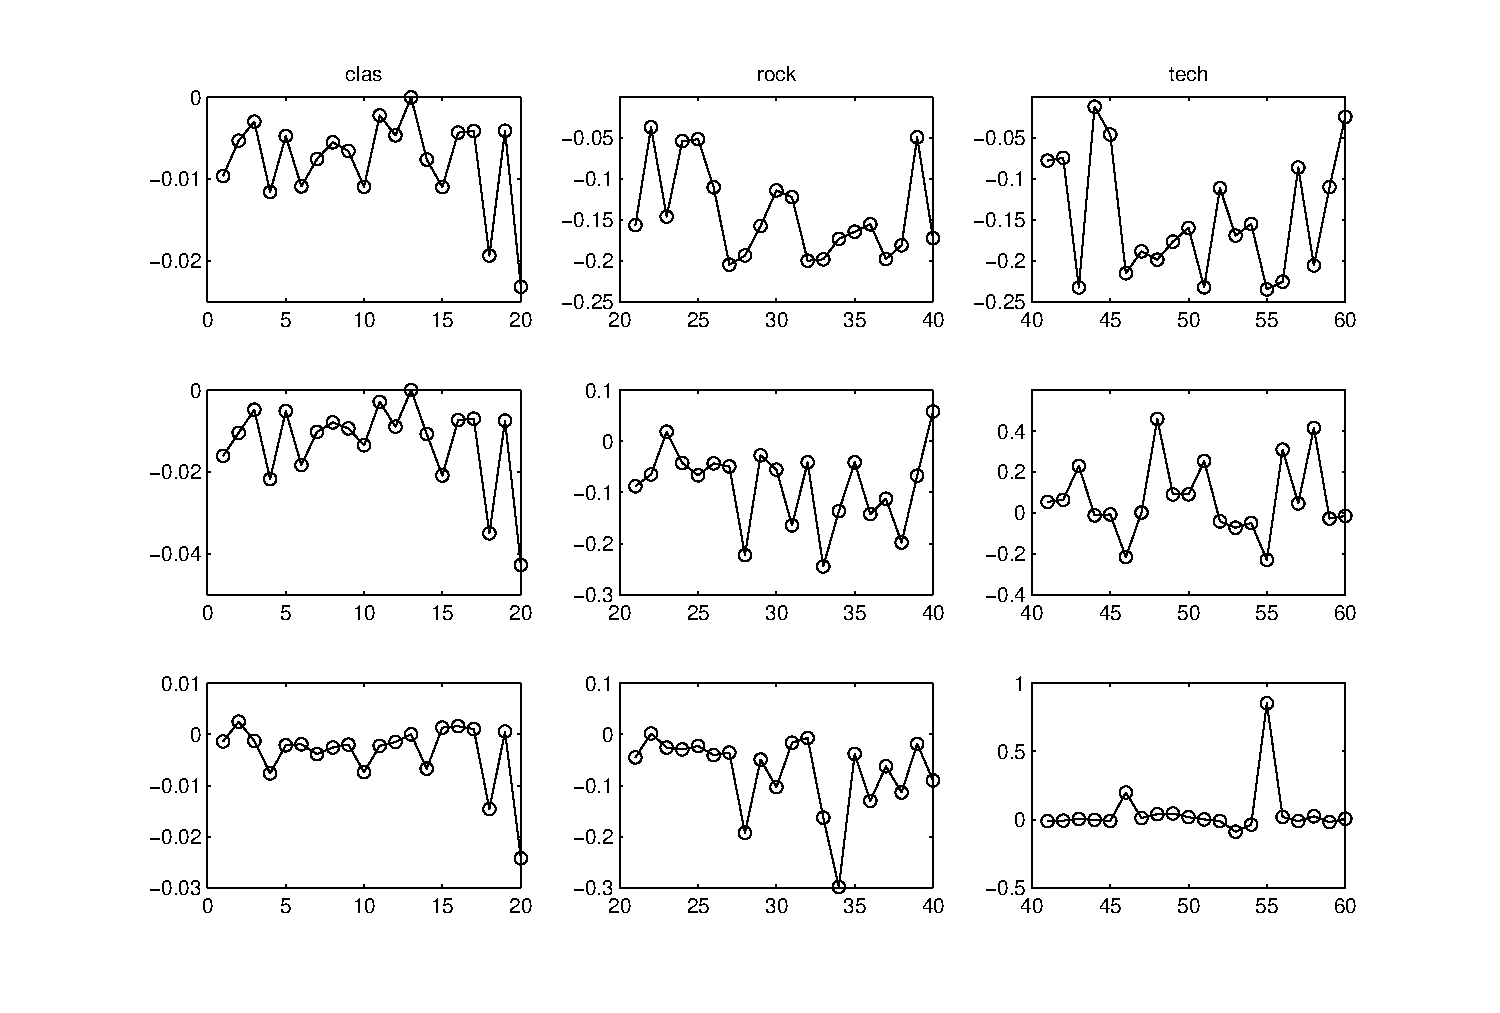
\includegraphics[width=0.85\columnwidth]{plot/test3/projections}\textbf{}\\
\textbf{}%
\begin{minipage}[t]{0.75\columnwidth}%
\textbf{Figure 14.} For Test 3, projection of the individual tracks
onto the first three POD modes shows high intra-genre variance and
distinct signatures for each genre: classical (left), modern rock
(center), and techno (right).%
\end{minipage}
\par\end{center}

\noindent \begin{center}
\pagebreak{}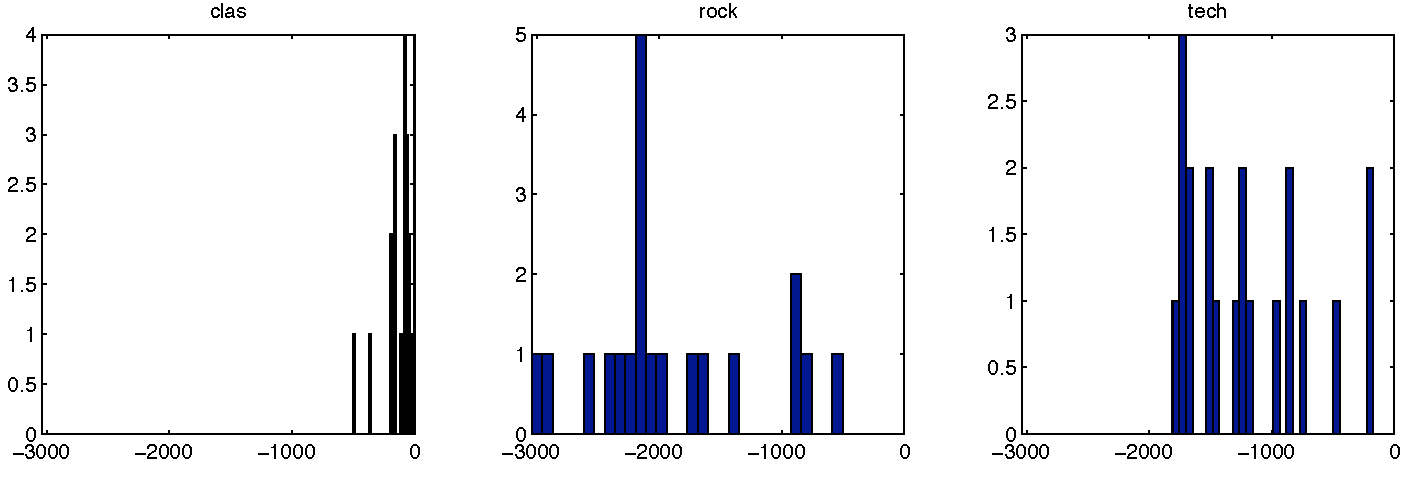
\includegraphics[width=0.95\columnwidth]{plot/test3/histogram}\textbf{}\\
\textbf{}%
\begin{minipage}[t]{0.75\columnwidth}%
\textbf{Figure 15.} For Test 3, histograms of the projections shows
high intra-genre variance and distinct signatures for each genre:
classical (left), modern rock (center), and techno (right)%
\end{minipage}\vspace{0.03\paperheight}
\par\end{center}

\section{Summary and Conclusions}

Ultimately, the objective in this project is to develop an algorithm
to classify music genre and bands based on their time-frequency signatures.
Using music from my iTunes collection, time-frequency analysis with
the G�bor transform, singular value decomposition (SVD) , and linear
discriminant analysis (LDA), this algorithm proves to be most effective
with band classification from different genres and struggled with
classification of different genres and bands within a single genre.

One limitation with this analysis is the number of tracks or data
points used in the tests and training sets. Though the results above
hint at the accuracy and performance of the algorithm, larger data
sets would provide a more effective metric. However, there are memory
management limitations to this algorithm and a balance is struck between
resampling the incoming data to reduce size, maximizing the number
of samples, and preventing memory overload in MATLAB. 

An integral part of this project is the exploration of the methods,
and so the number of time-frequency ``features'' (identified as
modes from the SVD) necessary for optimal classification is extensively
tested. One of the primary values of the SVD method is that it provides
low rank approximations for a given dataset. This algorithm is run
for 1, 2, 4, 6, 8, 10, 20, 30, 40, 50, and 60 ``features'' or modes.
Since the training set contains 60 tracks then using 60 modes corresponds
to a full rank. Interestingly, approximately 10 modes proved to be
the most effective for all three test conditions. This may be related
to some intrinsic structure of recorded music and further exploration
of this phenomena is an interesting application of this algorithm.

\section*{Appendix A (MATLAB functions)}
\begin{description}
\item [{diag}] Used to extract the diagonals from a matrix.
\item [{double}] Used to convert 8-bit integer image data to double precision
format.
\item [{eig}] Used to solve the eigenvalue problem; the function returns
the eigenvalues and eigenvectors used for the LDA.
\item [{fftn}] The all important FFT function, which performs a discritized
Fourier Transforms. This version of the function transforms $n$-dimensional
data. The $\mathtt{fft}$ and $\mathtt{fft}2$ versions transform
1- and 2-dimensional data respectively.
\item [{fftshift}] The output of the $\mathtt{fft}$ algorithm is shifted
(butterfly algorithm), so data in the frequency domain is shifted
back using this function before plotting.
\item [{frame2im}] Used to covert a movie frame to an image.
\item [{length}] Used to get the length of vectors.
\item [{load}] Loads data from an external file.
\item [{ind2sub}] Used to convert a linear index (in this case the minimum
value in the difference image) into corresponding 2D subscripts.
\item [{linspace}] Used to build a linear vector with $n+1$ points for
the spatial domain. The vector is then trimmed to $n$ points due
to the periodic boundaries.
\item [{max}] Used to find the maximum value in a given array.
\item [{mean}] Used to calculate the mean for each row of the location
coordinate data. 
\item [{num2str}] Used to convert a number to a string.
\item [{pcolor}] Used to plot the 3D spectrograms.
\item [{plot}] Used to plot the various parameters agains time or frequency.
\item [{repmat}] Used to replicate and tile an array for the means.
\item [{reshape}] Reshapes vector or matrix for given dimensions.
\item [{semilogy}] Used to make a plot with the $y$-axis on a logarithmic
scale.
\item [{size}] Used to get the number of rows and columns for a given matrix.
\item [{strcat}] Used to concatenate a string.
\item [{subplot}] Used to produce plot arrays.
\item [{sum}] Used to calculate sums.
\item [{svd}] The all important SVD function used to obtain the $U$, $S$,
and $V$ matrices.
\item [{switch}] Conditional structure used to vary code execution based
on a specified tag.
\item [{tic/toc}] Used to time the operations.
\item [{zeros}] Used to build vectors and matrices filled with ``0''.
\end{description}
\noindent \begin{center}
\pagebreak{}
\par\end{center}

\section*{Appendix B (code)}

See project root directory for scripts.

\subsection*{Main}

\noindent Main control script $\mathtt{main.m}$.

\subsection*{Gabor}

\noindent Subroutine $\mathtt{\left(gabor.m\right)}$ for the Gabor
Transform.

\subsection*{Trainer}

\noindent Subroutine $\mathtt{\left(trainer.m\right)}$ for building
the training set and LDA calculations.

\subsection*{Importing Data}

\noindent Subroutine $\mathtt{\left(loadTrack.m\right)}$ for importing
track data.

\subsection*{Plotting Frequency Data}

\noindent Subroutine $\mathtt{\left(plot\_freq.m\right)}$ for plotting
2D frequency data.

\subsection*{Plotting Histogram of Results}

\noindent Subroutine $\mathtt{\left(plot\_histo.m\right)}$ for plotting
LDA results.

\subsection*{Plotting LDA Results}

\noindent Subroutine $\mathtt{\left(plot\_lda.m\right)}$ for plotting
LDA results.

\subsection*{Plotting Spectrograms}

\noindent Subroutine $\mathtt{\left(plot\_spectro.m\right)}$ for
plotting spectrograms.

\section*{Appendix C (calculations)}

None

\section*{Appendix D (data)}

Here is the data obtained for the testing the ``features'' (modes)
parameter used for SVD/LDA:

\noindent \begin{center}
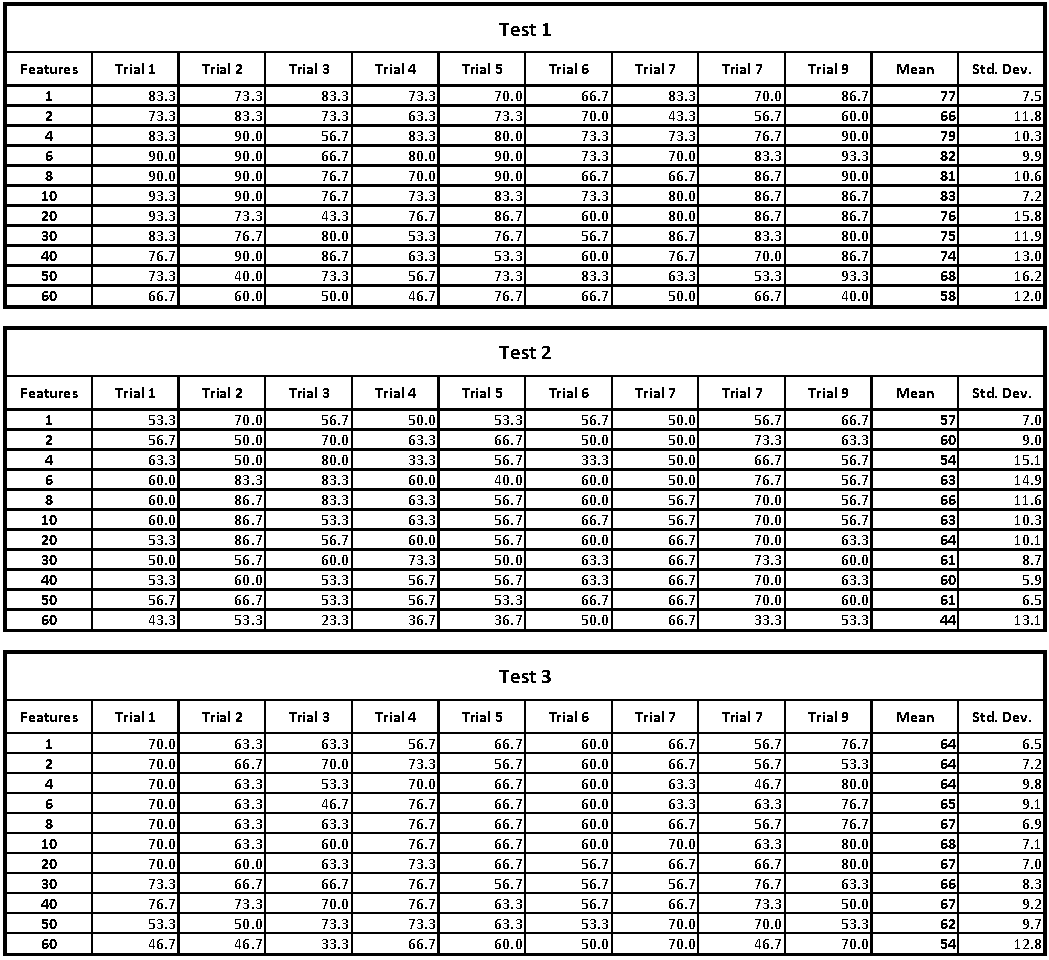
\includegraphics[width=0.95\columnwidth]{plot/results_all}
\par\end{center}
\end{document}
